\chapter{And then into Quantum Physics and Quantum Mechanics}


Let us start with the buckling beam. This is a two-point boundary
value problem
\[
R \frac{d^2 u(x)}{dx^2} = -F u(x),
\]
where $u(x)$ is the vertical displacement, $R$ is a material specific
constant, $F$ is the applied force and $x \in [0,L]$ with $u(0)=u(L)=0$.
We scale the equation with $x = \rho L$ and $\rho \in [0,1]$ and get
(note that we change from $u(x)$ to $v(\rho)$)
\[
\frac{d^2 v(\rho)}{dx^2} +K v(\rho)=0,
\]
which is, when discretized (see below), nothing but a standard eigenvalue problem with $K=
FL^2/R$. Here we can assume that either the force $F$ or the material
specific rigidity $R$ are unknown.  If we replace $R=-\hbar^2/2m$ and
$-F=\lambda$, we have the quantum mechanical variant for a particle
moving in a well with infinite walls at the endpoints.  The way to
solve these equations numerically is to discretize the second
derivative and the right hand side as
\[
    -\frac{v_{i+1} -2v_i +v_{i-i}}{h^2}=\lambda v_i,
\]
with $i=1,2,\dots, n$. Here $h$ is the step size which is defined by
the number of integration (or mesh) points.  We need to add to this
system the two boundary conditions $v(0) =v_0$ and $v(1) = v_{n+1}$,
although they are not needed in the solution of the equations since
their values are known.  For all integration points $i=1,2,\dots, n$
the set of equations to solve result in a so-called tridiagonal
Toeplitz matrix ( a special case from the discretized second
derivative)
\[
    \mathbf{A} = \frac{1}{h^2}\begin{bmatrix}
                          2 & -1 &  &   &  & \\
                          -1 & 2 & -1 & & & \\
                           & -1 & 2 & -1 & &  \\
                           & \dots   & \dots &\dots   &\dots & \dots \\
                           &   &  &-1  &2& -1 \\
                           &    &  &   &-1 & 2 \\
                      \end{bmatrix}
\]
and with the corresponding vectors $\mathbf{v} = (v_1, v_2,
\dots,v_n)^T$ allows us to rewrite the differential equation as a
standard eigenvalue problem
\[
   \mathbf{A}\mathbf{v} = \lambda\mathbf{v}.
\]
The tridiagonal Toeplitz matrix has analytical eigenpairs,
providing us thereby with an invaluable check on the equations to be
solved.

If we stay with quantum mechanical one-body problems (or
special interacting two-body problems) adding a potential along the
diagonal elements allows us to reuse this problem for many types of physics
cases.  To see this, let us assume we are interested in the solution
of the radial part of Schr\"odinger's equation for one electron. This
equation reads
\[
  -\frac{\hbar^2}{2 m} \left ( \frac{1}{r^2} \frac{d}{dr} r^2
  \frac{d}{dr} - \frac{l (l + 1)}{r^2} \right )R(r)
     + V(r) R(r) = E R(r).
\]
Suppose in our case $V(r)$ is the harmonic oscillator potential
$(1/2)kr^2$ with $k=m\omega^2$ and $E$ is the energy of the harmonic
oscillator in three dimensions.  The oscillator frequency is $\omega$
and the energies are
\[
E_{nl}=  \hbar \omega \left(2n+l+\frac{3}{2}\right),
\]
with $n=0,1,2,\dots$ and $l=0,1,2,\dots$.

Since we have made a transformation to spherical coordinates it means
that $r\in [0,\infty)$. The quantum number $l$ is the orbital momentum
  of the electron.  In order to find analytical solutions for this
  problem, we would substitute $R(r) = (1/r) u(r)$ (which gives
  $u(0)=u(\infty)=0$ and thereby easier boundary conditions) and
  obtain
\[
  -\frac{\hbar^2}{2 m} \frac{d^2}{dr^2} u(r)
       + \left ( V(r) + \frac{l (l + 1)}{r^2}\frac{\hbar^2}{2 m}
                                    \right ) u(r)  = E u(r) .
\]
The boundary conditions are $u(0)=0$ and $u(\infty)=0$.

In order to scale the equations, we introduce a dimensionless variable $\rho = (1/\alpha) r$
where $\alpha$ is a constant with dimension length and get
\[
  -\frac{\hbar^2}{2 m \alpha^2} \frac{d^2}{d\rho^2} v(\rho)
       + \left ( V(\rho) + \frac{l (l + 1)}{\rho^2}
         \frac{\hbar^2}{2 m\alpha^2} \right ) v(\rho)  = E v(\rho) .
\]
Let us choose $l=0$ for the mere sake of simplicity.
Inserting $V(\rho) = (1/2) k \alpha^2\rho^2$ we end up with
\[
  -\frac{\hbar^2}{2 m \alpha^2} \frac{d^2}{d\rho^2} v(\rho)
       + \frac{k}{2} \alpha^2\rho^2v(\rho)  = E v(\rho).
\]
We multiply thereafter with $2m\alpha^2/\hbar^2$ on both sides and obtain
\[
  -\frac{d^2}{d\rho^2} v(\rho)
       + \frac{mk}{\hbar^2} \alpha^4\rho^2v(\rho)  = \frac{2m\alpha^2}{\hbar^2}E v(\rho) .
\]

A natural length scale comes out automatically when scaling. To see this, since $\alpha$ is constant we are left to determine, 
we determine $\alpha$ by requiring that
\[
\frac{mk}{\hbar^2} \alpha^4 = 1.
\]
This defines a natural length scale in terms of the various physical
constants that determine the equation.  The final expression, inserting $k=m\omega^2$ is
\[
\alpha = \left(\frac{\hbar}{m\omega}\right)^{1/2}.
\]
If we were to replace the harmonic oscillator potential with the
attractive Coulomb interaction from the hydrogen atom, the  parameter $\alpha$ would equal the Bohr
radius $a_0$.  This way students see the general properties of a
two-point boundary value problem and can reuse the code they developed
for a mechanics course to the subsequent quantum mechanical course.

Defining
\[
\lambda = \frac{2m\alpha^2}{\hbar^2}E,
\]
we can rewrite Schroedinger's equation as
\[
  -\frac{d^2}{d\rho^2} v(\rho) + \rho^2v(\rho)  = \lambda v(\rho) .
\]
This is similar to the equation for a buckling beam, except for the
potential term.  In three dimensions with our scaling, the eigenvalues for $l=0$ are
$\lambda_0=3,\lambda_1=7,\lambda_2=11,\dots .$

If we  define first the diagonal matrix element
\[
   d_i=\frac{2}{h^2}+V_i,
\]
and the non-diagonal matrix element
\[
   e_i=-\frac{1}{h^2},
\]
we can rewrite the Schr\"oedinger equation as
\[
d_iu_i+e_{i-1}v_{i-1}+e_{i+1}v_{i+1}  = \lambda v_i,
\]
where $v_i$ is unknown and $i=1,2,\dots, n$. We can reformulate the
latter equation as a matrix eigenvalue problem
\[
    \begin{bmatrix} d_1 & e_1 & 0   & 0    & \dots  &0     & 0 \\
                                e_1 & d_2 & e_2 & 0    & \dots  &0     &0 \\
                                0   & e_2 & d_3 & e_3  &0       &\dots & 0\\
                                \dots  & \dots & \dots & \dots  &\dots      &\dots & \dots\\
                                0   & \dots & \dots & \dots  &\dots       &d_{n-1} & e_{n-1}\\
                                0   & \dots & \dots & \dots  &\dots       &e_{n-1} & d_{n}
             \end{bmatrix}      \begin{bmatrix} v_{1} \\
                                                              v_{2} \\
                                                              \dots\\ \dots\\ \dots\\
                                                              v_{n}
             \end{bmatrix}=\lambda \begin{bmatrix}{c} v_{1} \\
                                                              v_{2} \\
                                                              \dots\\ \dots\\ \dots\\
                                                              v_{n}
             \end{bmatrix}
\]
or if we wish to be more detailed, we can write the tridiagonal matrix as
\[
    \begin{bmatrix} \frac{2}{h^2}+V_1 & -\frac{1}{h^2} & 0   & 0    & \dots  &0     & 0 \\
                                -\frac{1}{h^2} & \frac{2}{h^2}+V_2 & -\frac{1}{h^2} & 0    & \dots  &0     &0 \\
                                0   & -\frac{1}{h^2} & \frac{2}{h^2}+V_3 & -\frac{1}{h^2}  &0       &\dots & 0\\
                                \dots  & \dots & \dots & \dots  &\dots      &\dots & \dots\\
                                0   & \dots & \dots & \dots  &\dots       &\frac{2}{h^2}+V_{n-1} & -\frac{1}{h^2}\\
                                0   & \dots & \dots & \dots  &\dots       &-\frac{1}{h^2} & \frac{2}{h^2}+V_{n}
             \end{bmatrix}.
\]

The following Python code sets up the matrix to diagonalize by defining
the minimun and maximum values of $r$ with a maximum value of
integration points. It plots the eigenfunctions of the three lowest
eigenstates.
\begin{lstlisting}
#Program which solves the one-particle Schrodinger equation
#for a potential specified in function
#potential().

from  matplotlib import pyplot as plt
import numpy as np
#Function for initialization of parameters
def initialize():
    RMin = 0.0
    RMax = 10.0
    lOrbital = 0
    Dim = 400
    return RMin, RMax, lOrbital, Dim
# Harmonic oscillator potential
def potential(r):
    return 0.5*r*r

#Get the boundary, orbital momentum and number of integration points
RMin, RMax, lOrbital, Dim = initialize()

#Initialize constants
Step    = RMax/(Dim)
DiagConst = 2.0/ (Step*Step)
NondiagConst =  -1.0 / (Step*Step)
OrbitalFactor = lOrbital * (lOrbital + 1.0)

#Calculate array of potential values
v = np.zeros(Dim)
r = np.linspace(RMin,RMax,Dim)
for i in range(Dim):
    r[i] = RMin + (i+1) * Step;
    v[i] = potential(r[i]) + OrbitalFactor/(r[i]*r[i]);

#Setting up a tridiagonal matrix and finding eigenvectors and eigenvalues
Matrix = np.zeros((Dim,Dim))
Matrix[0,0] = DiagConst + v[0];
Matrix[0,1] = NondiagConst;
for i in xrange(1,Dim-1):
    Matrix[i,i-1]  = NondiagConst;
    Matrix[i,i]    = DiagConst + v[i];
    Matrix[i,i+1]  = NondiagConst;
Matrix[Dim-1,Dim-2] = NondiagConst;
Matrix[Dim-1,Dim-1] = DiagConst + v[Dim-1];
# diagonalize and obtain eigenvalues, not necessarily sorted
EigValues, EigVectors = np.linalg.eig(Matrix)
# sort eigenvectors and eigenvalues
permute = EigValues.argsort()
EigValues = EigValues[permute]
EigVectors = EigVectors[:,permute]
# now plot the results for the three lowest lying eigenstates
for i in range(3):
    print(EigValues[i])
FirstEigvector = EigVectors[:,0]
SecondEigvector = EigVectors[:,1]
ThirdEigvector = EigVectors[:,2]
plt.plot(r, FirstEigvector**2 ,'b-',r, SecondEigvector**2 ,'g-',r, ThirdEigvector**2 ,'r-')
plt.axis([0,4.6,0.0, 0.025])
plt.xlabel(r'$r$')
plt.ylabel(r'Radial probability $r^2|R(r)|^2$')
plt.title(r'Radial probability distributions for three lowest-lying states')
plt.savefig('eigenvector.pdf')
plt.show()
\end{lstlisting}


The last example shows the potential of combining numerical algorithms with analytical results (or eventually symbolic calculations), allowing thereby students to test their physics understanding. One can easily switch to other potentials by simply redefining the potential function. For example, a finite box potential can easily be defined as
\begin{lstlisting}
# Finite depth and range box potential, with strength V and range a
def potential(r):
    if r >= 0.0 and r <= 10.0:
        V = -0.05
    else:
        V =0.0
    return V
\end{lstlisting}
Thereafter, the students can explore the role of the potential depth
and the range of the potential. Analyzing the eigenvectors gives
additional information about the spatial degrees of freedom in terms
of different potentials.  The possibility to visualize the results immediately, as shown in figure \ref{fig:eigenvector}, aids in providing students with a deeper understanding of the relevant physics.

This example contains also many of the
computing learning outcomes we discussed above, in addition to those
related to the physics of a particular system. We see that, by proper
scaling, the students can make further abstractions and explore other
physics cases easily where no analytical solutions are known. With
unit testing and analytical results they can validate and verify their
algorithms.
\begin{figure}
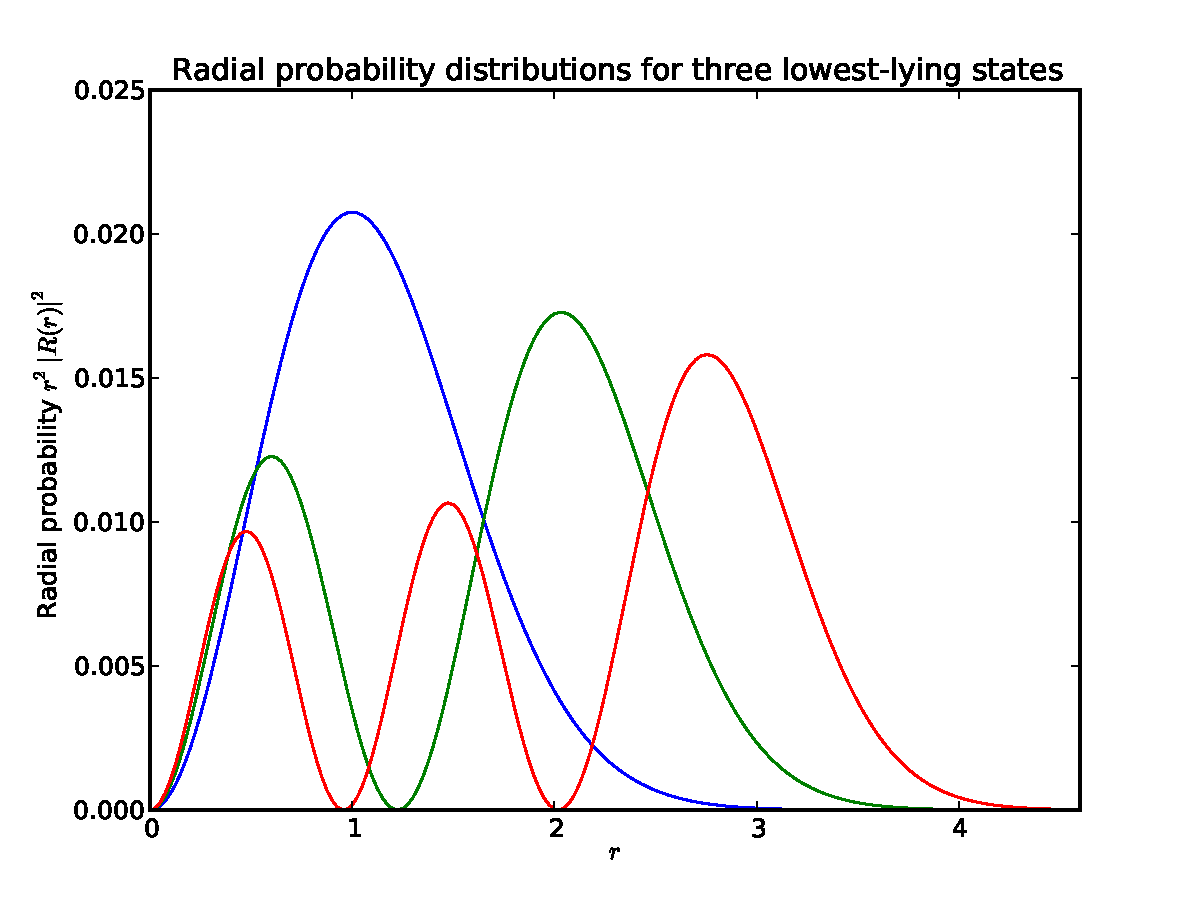
\includegraphics[scale=0.8]{Figures/eigenvector.pdf}
\caption{Plot of the eigenfunctions of the three lowest-lying eigenvalues for a harmonic oscillator problem in three dimensions. The students can easily change the type of potential and explore the physics that arises from these potentials.}\label{fig:eigenvector}
\end{figure}



The above example allows the student to test the mathematical error of
the algorithm for the eigenvalue solver by simply changing the number
of integration points. Again, as discussed above in connection with
the trapezoidal rule, the students get trained to develop an
understanding of the error analysis and where things can go wrong. The
algorithm can be tailored to any kind of one-particle problem used in
quantum mechanics.

